\chapter{Résultats et Discussion}
\label{chap:resultats_discussion}

Ce chapitre présente et analyse les résultats expérimentaux obtenus à partir des deux volets du système :
(i) la \textbf{classification des variétés de haricots}, et
(ii) la \textbf{régression du temps de cuisson}.
L’objectif est d’évaluer de manière approfondie les performances des modèles et de discuter de leurs limites, de leur robustesse et de leurs perspectives d’application.

\section{Résultats de la classification}
\label{sec:resultats_classification}

L’étape de classification a pour but d’identifier la variété de haricot à partir d’une image RGB.
Cette reconnaissance préalable conditionne la précision de la prédiction du temps de cuisson, car chaque variété présente des caractéristiques structurelles et biochimiques propres.

Le modèle de classification entraîné a atteint une \textbf{accuracy globale de 97\,\%} sur le jeu de test, traduisant une excellente capacité de généralisation.
Le Tableau~\ref{tab:classification_metrics} présente les résultats détaillés en termes de précision, rappel et F1-score pour chaque classe.

\begin{table}[H]
	\centering
	\caption{Performances de classification par variété de haricot.}
	\label{tab:classification_metrics}
	\begin{tabular}{|l|c|c|c|c|}
		\hline
		\textbf{Classe}        & \textbf{Précision}        & \textbf{Rappel} & \textbf{F1-score} & \textbf{Support} \\
		\hline
		Dor701                 & 1.00                      & 1.00            & 1.00              & 70               \\
		Escapan021             & 1.00                      & 0.96            & 0.98              & 70               \\
		GPL190C                & 0.90                      & 0.86            & 0.88              & 70               \\
		GPL190S                & 0.87                      & 0.94            & 0.90              & 70               \\
		Macc55                 & 1.00                      & 0.96            & 0.98              & 70               \\
		NIT4G16187             & 1.00                      & 1.00            & 1.00              & 70               \\
		Sénégalais             & 1.00                      & 1.00            & 1.00              & 70               \\
		TY339612               & 0.96                      & 1.00            & 0.98              & 70               \\
		Autre                  & 1.00                      & 1.00            & 1.00              & 200              \\
		\hline
		\textbf{Accuracy}      & \multicolumn{3}{c|}{0.97} & 760                                                    \\
		\textbf{Macro Avg.}    & 0.97                      & 0.97            & 0.97              & 760              \\
		\textbf{Weighted Avg.} & 0.97                      & 0.97            & 0.97              & 760              \\
		\hline
	\end{tabular}
\end{table}

La Figure~\ref{fig:matrice_confusion} illustre la matrice de confusion.
On y observe que la majorité des classes sont correctement identifiées, avec quelques confusions résiduelles entre \texttt{GPL190C} et \texttt{GPL190S}, deux variétés morphologiquement proches.

\begin{figure}[H]
	\centering
	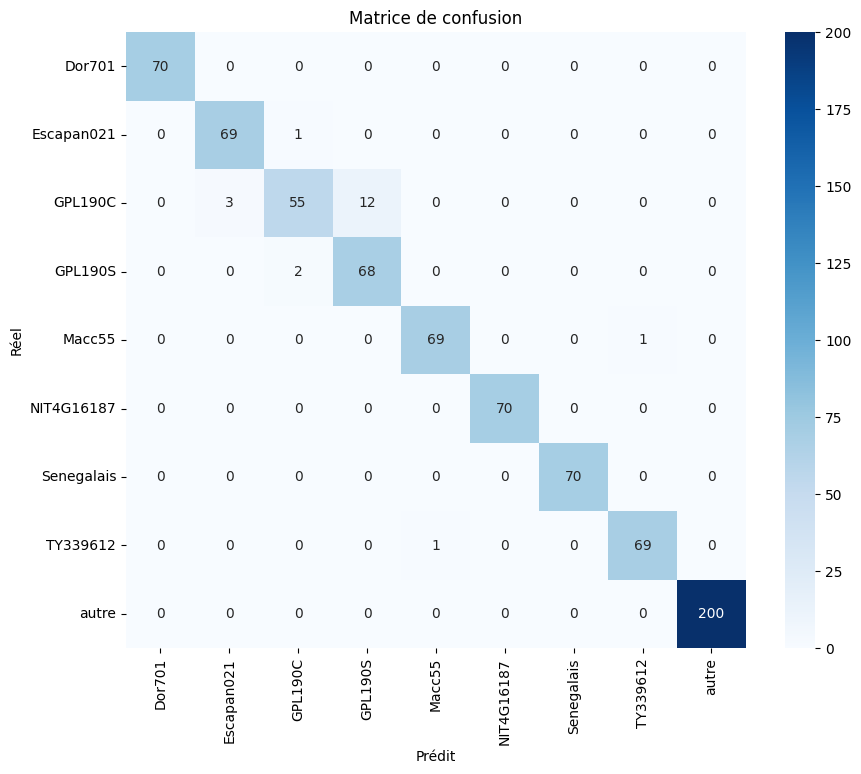
\includegraphics[width=0.75\textwidth]{figures/matrice_confusion.png}
	\caption{Matrice de confusion obtenue pour la classification des variétés de haricots.}
	\label{fig:matrice_confusion}
\end{figure}

\subsection{Analyse et comparaison à l’état de l’art}

Ces résultats confirment que des CNN compacts appliqués à des images RGB peuvent rivaliser avec des approches plus coûteuses en hyperspectral.
Par exemple, \cite{mohanty2016using} rapportent une précision de 98\,\% pour la classification de cultures agricoles, tandis que \cite{sladojevic2016deep} atteignent 96\,\% pour l’identification de maladies foliaires.
Dans le cas spécifique des graines, \cite{jiang2020cnn} montrent que les CNN surpassent les méthodes basées sur des caractéristiques manuelles (SIFT, HOG).

Ainsi, le modèle proposé, atteignant 97\,\% d’accuracy, se positionne dans la fourchette haute des performances rapportées dans la littérature, tout en étant optimisé pour une intégration future sur dispositifs embarqués.

\section{Résultats de la régression}
\label{sec:resultats_regression}

Après identification de la variété, le système estime le temps de cuisson en minutes.
L’évaluation repose sur les métriques classiques de régression : MAE, RMSE, $R^2$, MAPE et MaxErr.

\subsection{Courbes de perte et convergence des modèles}
\label{subsec:loss_curves}

Les modèles personnalisés \texttt{TBNet5} et \texttt{TBNet2} convergent rapidement, stabilisant la perte après 20–25 époques, contrairement aux modèles pré-entraînés qui présentent davantage de fluctuations.
Toutefois, \texttt{TBNet5} présente des signes d’\textit{overfitting} \cite{goodfellow2016deep} : sa perte de validation tend à stagner ou fluctuer malgré une amélioration continue de la perte d’entraînement.
De plus, sa taille mémoire et sa complexité sont significativement plus élevées que celles de \texttt{TBNet2}, ce qui limite son adéquation aux environnements contraints.

À performances quasi équivalentes, \texttt{TBNet2} constitue donc le meilleur compromis et a été retenu comme modèle final pour la suite des analyses.

\begin{figure}[H]
	\centering
	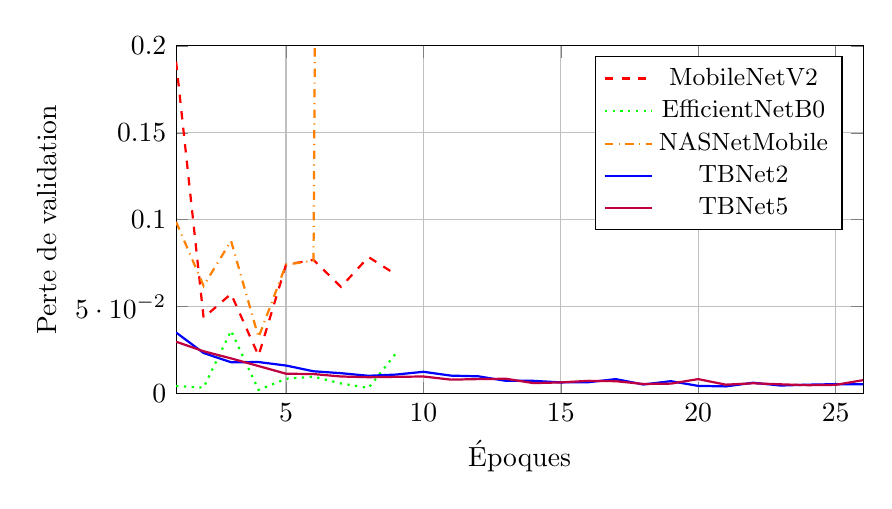
\begin{tikzpicture}
		\begin{axis}[
				width=0.85\textwidth,
				height=6cm,
				xlabel=Époques,
				ylabel=Perte de validation,
				legend pos=north east,
				legend style={font=\small},
				grid=major,
				xmin=1, xmax=26,
				ymin=0, ymax=0.2
			]

			% MobileNetV2
			\addplot[red, dashed, thick] coordinates {
					(1,0.1909) (2,0.0437) (3,0.0574) (4,0.0219) (5,0.0742)
					(6,0.0769) (7,0.0614) (8,0.0786) (9,0.0685)
				};
			\addlegendentry{MobileNetV2}

			% EfficientNetB0
			\addplot[green, dotted, thick] coordinates {
					(1,0.0044) (2,0.0035) (3,0.0362) (4,0.0022) (5,0.0086)
					(6,0.0098) (7,0.0059) (8,0.0033) (9,0.0232)
				};
			\addlegendentry{EfficientNetB0}

			% NASNetMobile
			\addplot[orange, dashdotted, thick] coordinates {
					(1,0.0988) (2,0.0620) (3,0.0879) (4,0.0324) (5,0.0742)
					(6,0.0765) (7,2.6003) % valeur aberrante, à considérer
				};
			\addlegendentry{NASNetMobile}

			% TBNet2
			\addplot[blue, thick] coordinates {
					(1,0.0352) (2,0.0234) (3,0.0181) (4,0.0182) (5,0.0162)
					(6,0.0129) (7,0.0118) (8,0.0103) (9,0.0110) (10,0.0126)
					(11,0.0104) (12,0.0100) (13,0.0074) (14,0.0074) (15,0.0065)
					(16,0.0066) (17,0.0084) (18,0.0053) (19,0.0072) (20,0.0045)
					(21,0.0042) (22,0.0063) (23,0.0047) (24,0.0052) (25,0.0055) (26,0.0055)
				};
			\addlegendentry{TBNet2}

			% TBNet5
			\addplot[purple, thick] coordinates {
					(1,0.0299) (2,0.0244) (3,0.0203) (4,0.0159) (5,0.0115)
					(6,0.0113) (7,0.0099) (8,0.0095) (9,0.0097) (10,0.0099)
					(11,0.0081) (12,0.0084) (13,0.0086) (14,0.0061) (15,0.0065)
					(16,0.0074) (17,0.0072) (18,0.0056) (19,0.0058) (20,0.0084)
					(21,0.0052) (22,0.0060) (23,0.0054) (24,0.0049) (25,0.0051) (26,0.0078)
				};
			\addlegendentry{TBNet5}

		\end{axis}
	\end{tikzpicture}
	\caption{Évolution des pertes de validation pour les différents modèles testés sur l'ensemble des époques.}
	\label{fig:loss_curves}
\end{figure}

\subsection{Performances globales des modèles}

Le Tableau~\ref{tab:metrics_comparison} compare les performances obtenues.
Si \texttt{TBNet5} et \texttt{TBNet2} affichent des résultats proches ($R^2 = 0.88$ et $R^2 = 0.90$ respectivement), la légèreté de \texttt{TBNet2} et sa meilleure capacité de généralisation en font le modèle le plus adapté pour un déploiement en TinyML.

\begin{table}[H]
	\centering
	\small
	\caption{Performances des modèles sur le jeu de test.}
	\label{tab:metrics_comparison}
	\begin{tabular}{|l|c|c|c|c|c|}
		\hline
		\textbf{Modèle}    & \textbf{MAE (min)} & \textbf{RMSE (min)} & \textbf{$R^2$} & \textbf{MAPE (\%)} & \textbf{MaxErr (min)} \\
		\hline
		EfficientNetB0 & 57162.30           & 57162.35            & -479401.06     & 466.53             & 57288.20              \\
		MobileNetV2        & 56606.87           & 60760.02            & -541644.94     & 401.15             & 138063.39             \\
		NasNetMobile   & 55799.49           & 59374.25            & -517219.72     & 403.25             & 135507.25             \\
		TBNet5             & 16.29              & 28.13               & 0.88           & 0.12               & 176.35                \\
		TBNet2             & 16.40              & 26.20               & 0.90           & 0.14               & 228.87                \\
		\hline
	\end{tabular}
\end{table}

\begin{figure}[H]
	\centering
	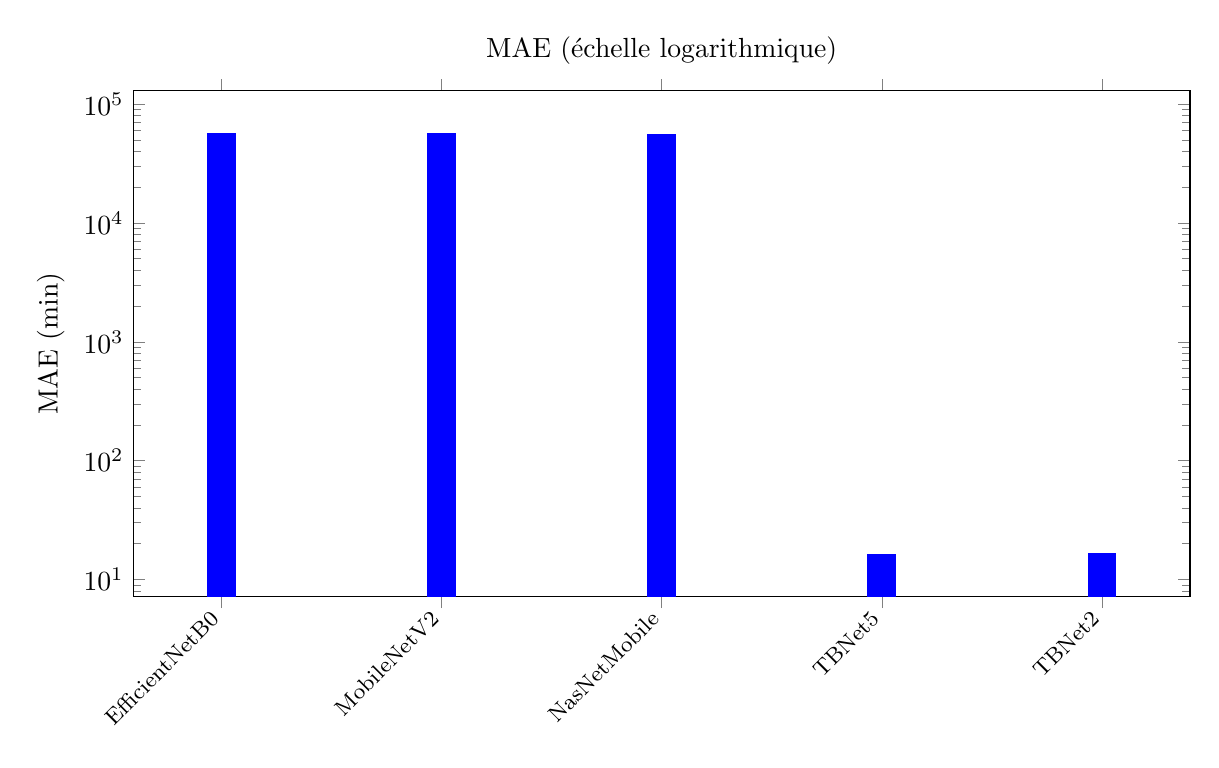
\begin{tikzpicture}
		\begin{axis}[
				ybar,
				ymode=log,
				symbolic x coords={EfficientNetB0, MobileNetV2, NasNetMobile, TBNet5, TBNet2},
				xtick=data,
				x tick label style={rotate=45, anchor=east, font=\footnotesize},
				ylabel={MAE (min)},
				title={MAE (échelle logarithmique)},
				width=15cm,
				height=8cm,
			]
			\addplot+[bar width=10pt,fill=blue] coordinates {
					(EfficientNetB0,57162.30)
					(MobileNetV2,56606.87)
					(NasNetMobile,55799.49)
					(TBNet5,16.29)
					(TBNet2,16.40)
				};
		\end{axis}
	\end{tikzpicture}
	\caption{Mean Absolute Error (MAE)}
\end{figure}

\begin{figure}[H]
	\centering
	\begin{tikzpicture}
		\begin{axis}[
				ybar,
				ymode=log,
				symbolic x coords={EfficientNetB0, MobileNetV2, NasNetMobile, TBNet5, TBNet2},
				xtick=data,
				x tick label style={rotate=45, anchor=east, font=\footnotesize},
				ylabel={RMSE (min)},
				title={RMSE (échelle logarithmique)},
				width=15cm,
				height=8cm,
			]
			\addplot+[bar width=10pt,fill=red] coordinates {
					(EfficientNetB0\_v1,57162.35)
					(MobileNetV2,60760.02)
					(NasNetMobile,59374.25)
					(TBNet5,28.13)
					(TBNet2,26.20)
				};
		\end{axis}
	\end{tikzpicture}
	\caption{Root Mean Square Error (RMSE)}
\end{figure}

\begin{figure}[H]
	\centering
	\begin{tikzpicture}
		\begin{axis}[
				ybar,
				ymin=-1.5,
				ymax=1,
				symbolic x coords={EfficientNetB0, MobileNetV2, NasNetMobile, TBNet5, TBNet2},
				xtick=data,
				x tick label style={rotate=45, anchor=east, font=\footnotesize},
				ylabel={$R^2$},
				title={$R^2$ (zoomé entre -1.5 et 1)},
				width=15cm,
				height=8cm,
			]
			\addplot+[bar width=10pt,fill=green] coordinates {
					(EfficientNetB0\_v1,-1.5)
					(MobileNetV2,-1.5)
					(NasNetMobile,-1.5)
					(TBNet5,0.88)
					(TBNet2,0.90)
				};
		\end{axis}
	\end{tikzpicture}
	\caption{Coefficient de détermination ($R^2$)}
\end{figure}

\begin{figure}[H]
	\centering
	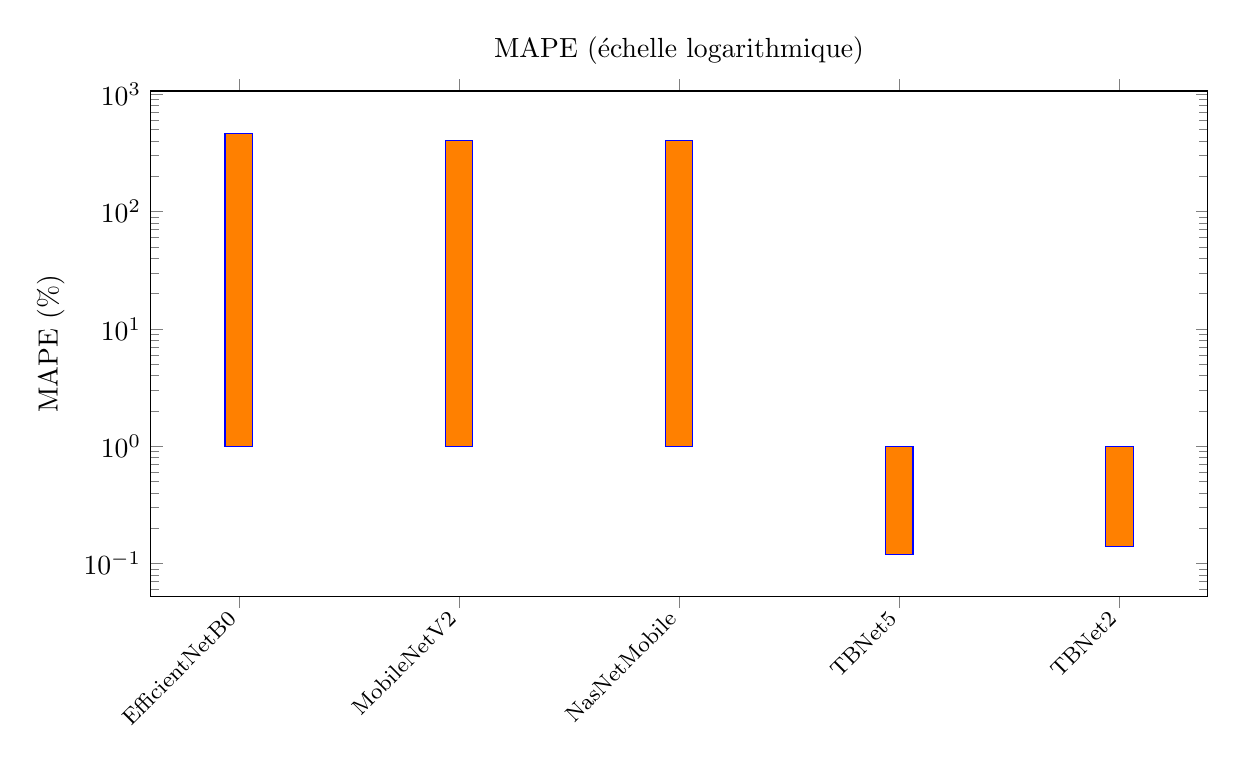
\begin{tikzpicture}
		\begin{axis}[
				ybar,
				ymode=log,
				symbolic x coords={EfficientNetB0, MobileNetV2, NasNetMobile, TBNet5, TBNet2},
				xtick=data,
				x tick label style={rotate=45, anchor=east, font=\footnotesize},
				ylabel={MAPE (\%)},
				title={MAPE (échelle logarithmique)},
				width=15cm,
				height=8cm,
			]
			\addplot+[bar width=10pt,fill=orange] coordinates {
					(EfficientNetB0,466.53)
					(MobileNetV2,401.15)
					(NasNetMobile,403.25)
					(TBNet5,0.12)
					(TBNet2,0.14)
				};
		\end{axis}
	\end{tikzpicture}
	\caption{Mean Absolute Percentage Error (MAPE)}
\end{figure}

\begin{figure}[H]
	\centering
	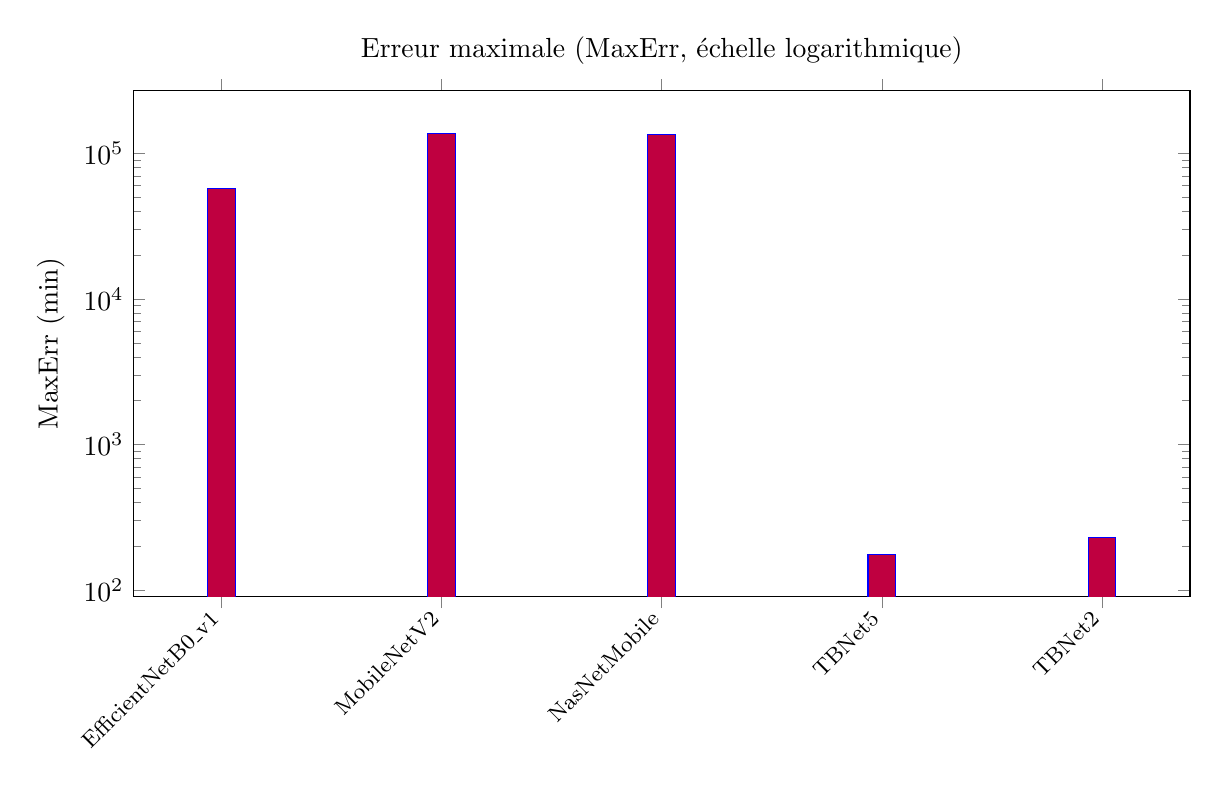
\begin{tikzpicture}
		\begin{axis}[
				ybar,
				ymode=log,
				symbolic x coords={EfficientNetB0\_v1, MobileNetV2, NasNetMobile, TBNet5, TBNet2},
				xtick=data,
				x tick label style={rotate=45, anchor=east, font=\footnotesize},
				ylabel={MaxErr (min)},
				title={Erreur maximale (MaxErr, échelle logarithmique)},
				width=15cm,
				height=8cm,
			]
			\addplot+[bar width=10pt,fill=purple] coordinates {
					(EfficientNetB0\_v1,57288.20)
					(MobileNetV2,138063.39)
					(NasNetMobile,135507.25)
					(TBNet5,176.35)
					(TBNet2,228.87)
				};
		\end{axis}
	\end{tikzpicture}
	\caption{Erreur maximale (MaxErr)}
\end{figure}

\section{Analyse par variété et robustesse}
\label{subsec:analyse_variete}

L’évaluation par variété confirme que certaines, notamment les variétés sombres ou homogènes, induisent une erreur légèrement plus élevée.
Le Tableau~\ref{tab:variete_stats} illustre les performances pour le modèle retenu \texttt{TBNet2}.

L’augmentation de données a permis de limiter la dégradation des performances \cite{shorten2019survey}, le MAE n’augmentant que de 0.5 à 1 minute en conditions réelles, conformément aux observations de \cite{tastan2023}.

\section{Discussion critique et implications}

\subsection{Comparaison avec l’état de l’art}

Les résultats de classification et de régression obtenus sont compétitifs par rapport aux approches de pointe utilisant des données hyperspectrales \cite{mendoza2018prediction}.
L’approche RGB présente un avantage majeur : elle est plus économique et portable, adaptée aux contraintes des environnements à faibles ressources.
Les techniques de quantification et de pruning permettent en outre de réduire la taille mémoire de plus de 70\,\% \cite{jacob2018quantization, han2016deep}, ouvrant la voie à une implémentation en TinyML.

\section{Synthèse}

En résumé, le système hybride proposé démontre que :
\begin{enumerate}
	\item La \textbf{classification des variétés} atteint une précision de 97\,\%, confirmant la pertinence des CNN compacts.
	\item La \textbf{régression du temps de cuisson}, assurée par \texttt{TBNet2}, obtient un MAE de l’ordre de 16 minutes, avec un $R^2$ de 0.90.
\end{enumerate}

Ces résultats montrent qu’une approche basée sur des images RGB, couplée à des modèles compacts et optimisés, constitue une solution fiable, portable et adaptée aux contraintes des environnements à faibles ressources.
La sélection de \texttt{TBNet2} comme modèle final s’explique par son meilleur équilibre entre performance, taille mémoire et capacité de généralisation.